\documentclass[english]{article}

\usepackage{babel}
\usepackage{graphicx}
\usepackage{alltt}
\usepackage{url}
\usepackage{tabularx}
%\usepackage{ngerman}
\usepackage{longtable}
\usepackage{color}
\usepackage{framed}
\usepackage{hyperref}
\usepackage{todonotes}


\usepackage{xifthen}
\newboolean{showbackdoors}
\setboolean{showbackdoors}{true}  % set to false to hide subsection on backdoors for reviewing group


\newenvironment{prettytablex}[1]{\vspace{0.3cm}\noindent\tabularx{\linewidth}{@{\hspace{\parindent}}#1@{}}}{\endtabularx\vspace{0.3cm}}
%\newenvironment{prettytable}{\prettytablex{l X}}{\endprettytablex}



\title{\huge\sffamily\bfseries System Description and Risk Analysis}
\author{Luca Di Bartolomeo \and Al\'{i}  El Wahsh \and Anselme Goetschmann \and Andreas Pfefferle}
\date{\today}


\begin{document}
\maketitle

%% **** please observe the page limit ****
%% (it is not allowed to change the font size or page geometry to gain more space)
%% comment or remove lines below before hand-in
%%\begin{center}
%%{\large\textcolor{red}{Page limit: 30 pages.}}
%%\end{center}
%%%%%%%%%%%%%%%%%%%%%%%%%%%%%%%%%%%%%%%%%%%%%%

\setcounter{tocdepth}{2}
\tableofcontents
\pagebreak


\section{System Characterization}

\subsection{System Overview}

The system we describe in this report acts as a certificate authority for the employees of the company iMovies. The employees can log in with their credentials or certificate to manage their personal information as well as their keys. It also provides an administration interface showing the number of active and revoked certificates.

The system is divided into the following parts, represented in figure \ref{overview}: the firewall, the web server, the CA core, the database and finally the backup. To allow the system administrator(s) (sysadmin) to access and manage the different parts, a dedicated administration server is also connected to all the machines via a management network.

When an employee wants to access the service, they connect to the web server through the firewall. The web server then performs the requests needed to the API provided by the CA core, which in turn queries the database. The access for the CA administrator(s) (CA admin) is similar.

To save the current state of the system, the backup server regularly queries the database and creates an encrypted archive. The logs from all the other machines are also redirected to the backup server and included in this archive.

When the system needs to be updated or maintained, the sysadmin securely connects to the admin server, from which they can perform the required actions.

\begin{figure}
  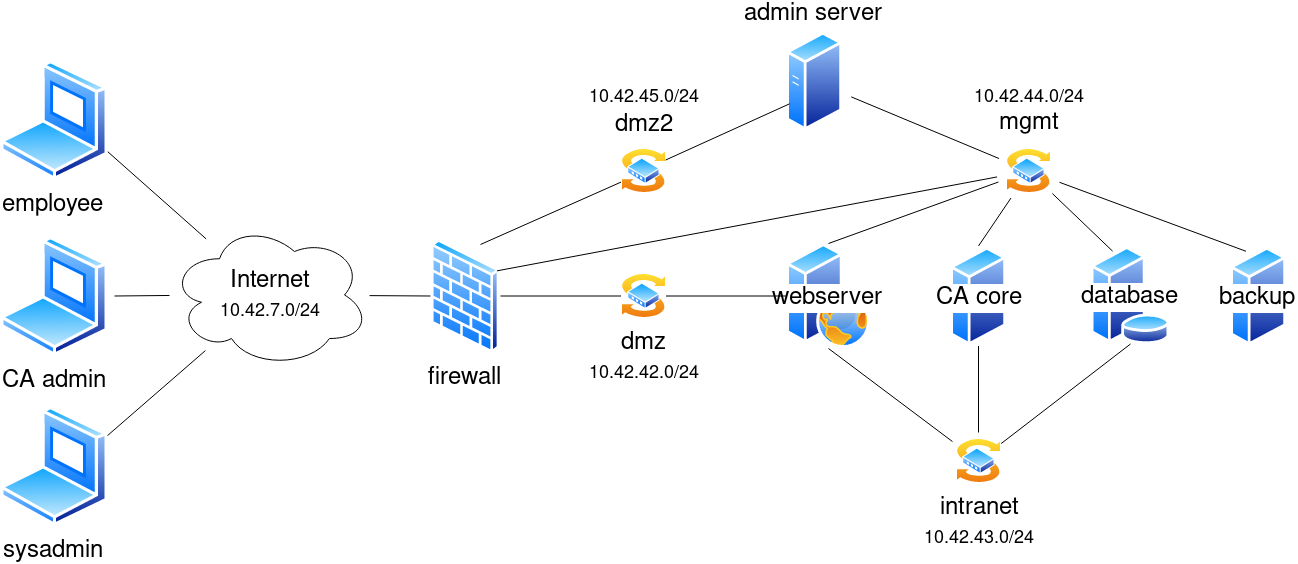
\includegraphics[width=\textwidth]{diagram.png}
  \caption{Overview of the CA system}
  \label{overview}
\end{figure}



\subsection{System Functionality}

In this section we describe the functionalities the system provides to the iMovies employees, CA admins and sysadmins.

\begin{itemize}
  \item \textbf{Employee - } An employee can access the system after having authenticated, either with their user name and password or with a valid certificate once they have one. The web interface shows the employee's personal information and provides the possibility to edit their name and email. The employee can also view a list of their valid and revoked certificates, create a new certificate and revoke an existing one. An employee cannot view, create, modify or delete anything else, only this limited set of privileges is granted to them. Therefore, this can be seen as an example for the least privilege principles and the usability principle (more options would confuse a user which leads to a weaker system). When a certificate has been revoked, the employee is not able to log in with it anymore.
  \item \textbf{CA admin - } A CA admin can connect with a valid certificate and consult the system's current state, which is summarised by the number of issued and revoked certificates and the serial number. The CA admin does not have any other privileges. This is an example of the least privilege principle.
  \todo{have to say somewhere that the ca admin cert is in the home folder}
  \item \textbf{Sysadmin - } A sysadmin can log in to the admin server via a secure shell with a SSH key which is secured with a very strong password. This is more secure than a SSH password alone, since it requires a) the possesion of the key and b) the knowledge of the password to login to the admin server. This is an example of the defense-in-depth and the no single point of failure principle. The passwords are randomly generated, are over 40 characters long and include special characters such as "\$". This is the application of security principle 1.3.11 Generating Secrets from the ASL book, which states that you should maximize the entropy of secrets. The passwords are stored in a password manager such that the sysadmin does not have to remember a lot of complex passwords, which is the application of principle 1.3.1 from the ASL book, which says that you should design usable security mechanisms. From the admin server, a command line interface allows them to configure and restart the firewall, web server, CA core, database and backup server. Again, the sysadmin uses SSH keys (one for each machine) that are stored on the admin server and are secured with a unique, very strong password that is stored in the password manager (the same techniques and principles as earlier in this section about SSH keys and passwords apply here). The overall access procedures for the sysadmin can be seen as an application of the principles of compartmentalization and minimum exposure. Also, since we don't invent any new authentication procedures by ourselves but instead use open protocols (like SSH) that rely on strong secrets (keys + passwords), you can also find the open design and the simplicity principle here.
\end{itemize}

\subsection{Components}
\label{Components}

\todo{I think it would be useful to introduce the networks first: dmz is for access to web interface from user, dmz2 is for sysadmin access to admin server, mgmt is for sysadmin access to hosts and logs, intranet is for requests between component to answer a user query}

\begin{itemize}
	\item \textbf{The client - } The client is modeled as any modern browser that connects through the internet to our firewall and establishes a TLS connection. \todo{I guess say that we use ubuntu/firefox} It doesn't have access to the other components of the system and is able to talk to the webserver through port 443 only. \todo{the sysadmin can also ssh}
	\item \textbf{The firewall -} The firewall machine filters traffic between the webserver and the public internet. It is a \emph{stateless} firewall that allows only inbound connections to port 443 (HTTPS) on the webserver and outbound connections from port 443 of the webserver. \todo{port 22 goes to adminserver} It is implemented using \texttt{iptables} rules.
		We chose a stateless firewall instead of a stateful one to avoid increasing the attack surface of our system and to avoid putting too much load on a single machine that could increase the overall latency of our system.
	\item \textbf{The webserver -} The server answering HTTP queries is implemented using \texttt{Apache} for dealing with connections and parsing headers and \texttt{Python Flask} for serving the frontend and managing the logic of the server. This machine is able to communicate to the outside Internet through the firewall machine; moreover it has an additional network interface linked to the "intranet" network that lets the webserver communicate with the core CA, the database and the backup machines. \todo{backup only for logging}  \\
		The webserver is able to authenticate a client based on its certificate, and for this reason it keeps a list of all generated public keys. \todo{no, it only has the CA cert (and checks that the client cert was signed with it) and a certification revocation list updated from the core at every revocation} Apart from that, it won't deal with any other operation involving certificates: creating and revoking queries are forwarded to the core CA machine through an internal API.  \\
		The webserver is able to read from the database, in order to authenticate clients based on the hash of their password; the webserver doesn't have write access to the database. Queries related to the changing of client's information (name, password, etc) are forwarded to the core CA machine through an internal API. \\
		The webserver logs every request it receives and every answer it produces, and will periodically send this logs to the backup machine.
		Finally, the webserver will be attached to another internal network, the "management", from where an admin can log in through SSH and have complete access to the machine.
	\item \textbf{The database machine -} This machine is responsible to keep track of the clients' information. For each client, it stores their email, name, ID and hashed (SHA-1) password. It is implemented using \texttt{MySQL}. \\
		The database gives read access to the webserver machine that connects through the "intranet" network. It gives read/write access to the core CA machine that connects through the "intranet" network.\todo{say precisely which requests from where: webserver: query user for login and info, query certificates for list display; core: update userinfo, insert cert, read private key for download, write for cert revocation} \\
		The database keeps a log of every query it receives and will periodically send the logs to the backup machine. \\
		The database is attached to another internal network, "management", from which an admin can log in through SSH and have complete access to the machine.
	\item \textbf{The backup machine -} The backup machine is responsible to keep an encrypted log of everything relevant that happens in the system, in order to restore a previous state in case any problems arise and additionally to understand what caused said problem. We haven't decided yet how to implement the backup system. \\
		The backup machine is attached to the "intranet" \todo{no, mgmt} network, and will accept logs from the firewall, webserver, core CA and database. Every information received will be appended to the backup - it will not be possible to overwrite data. Furthermore, since the backup contains very sensitive data such as private keys and passwords it must encrypt everything before storing. Data will be encrypted with a public key present on the backup machine. The corresponding private key to decrypt the backup will be given only to the system administrator.\\
		The backup machine is linked to an additional internal network, "management", from which the system administrator can log in through SSH and have complete control over the machine.
    \todo{database also periodically sends database dump (so push), which is encrypted the same way}
	\item \textbf{The core CA - } The core CA machine is the one who takes care of the generation and revocation of certificates. It exposes an API \todo{I guess we should explicitely give the API/endpoints} on the "intranet" network from which the webserver can ask for the generation or the revocation of a certificate, or for a change of a given client's information. The core CA then translates requests in a \texttt{SQL} query and forwards it to the database machine. The API will be implemented using \texttt{Python sockets}. \\
		The core CA machine is linked to an additional internal network, "management", from which the system administrator can log in through SSH and have complete control over the machine.
	\item \textbf{The admin server -} This machine will expose and SSH daemon to the internet, from which a system administrator can login and have access to the "management" network and fix any problems that can arise in any machine of our system. The sole purpose of this server is to avoid making every other machine expose an interface to the outside internet to permit SSH login.
  \todo{we could put this one after the firewall and remove the part about the mgmt net in each component. move the implementation details (what keys where) from 1.2 here}
\end{itemize}


\subsection{Security Design}

Here we discuss the security principles that we kept in mind while designing the system:

\begin{itemize}
	\item \textbf{Confidentiality}: client's data such as email, name, ID, and public keys will be displayed only over a successful login. We don't keep track of clear text passwords, and hashes won't be displayed over HTTP. We enforce having access only to port 443 from the internet and sanitization of all fields on the webserver to be sure of our confidentiality guarantee. Furthermore, private keys are only kept encrypted inside the backup machine, and the only way of seeing them is logging in through SSH and decrypting them with the administrator's private key.
	\item \textbf{Integrity}: We protect the integrity of the data inside the database by restricting write access to only the core CA machine, which can be accessed from the webserver only through a limited API. Instead, we guarantee the integrity of data in the backup by enforcing an append-only policy.
	\item \textbf{Availability}: We decided against complex IPS/IDS frameworks and in favour of a simple stateless firewall to ensure that the latency of our system stays low and traffic can flow in and out in a relatively fast way. We are still looking into ways to defend against potential Denial-of-Service attacks on our webserver.
	\item \textbf{Compartmentalization}: Every machine takes care of a single, necessary task. We avoided running multiple services on a single machine, with the exception of the SSH daemon for admin access.
	\item \textbf{Least privilege}: The read-only limits enforced to the webserver on the database queries and the fact that most of the services are listening only on the "intranet" interface are to limit privileges that each machine has.
	\item \textbf{Economy of mechanism, Simplicity}: The firewall is simple as possible, and custom implemented software (such as internal APIs) are implemented using Python, an understandable and memory safe language to minimize bugs.
	\item \textbf{Complete mediation}: All request coming from the internet must pass either through the webserver, or the admin server, and in both cases they need to be authenticated to modify the state of our system.
	\item \textbf{Separation of privilege}: All the machines in the "intranet" network can be accessed through SSH only through a previous SSH login on the admin server machine. Furthermore, a write operation on the database will be executed only if sent by the core CA which approved a request from the webserver.
\end{itemize}

\ifthenelse{\boolean{showbackdoors}}{
% show for handed-in version

\subsection{Backdoors}

\subsubsection*{Backdoor 1}
The webpage \texttt{html/crt/admin\_list.php} is accessible only by admins, and
lists all generated certificates in the database.  For every certificate, it
shows the login name of the user that generated it, the plaintext certificate,
and the private key of that certificate.  

This page is only accessible by admins, but a malicious user could exploit the
fact that the certificate is displayed in plaintext and execute an XSS
injection.  The user just needs to set up one of his personal information, such
as the email, to a string like the following:

\noindent
\texttt{<script>alert("XSS\_injected");<\textbackslash/script>}

The backslash of the closing tab \texttt{<\textbackslash/script>} is because
\texttt{openssl} will parse the email as the subject line of the certificate,
using forward slash as separator for fields. By escaping the forward slash, we
avoid that openssl mangles our paylods.

Since the email is displayed in the certificate, when an admin will access the
page \texttt{html/crt/admin\_list.php}, the javascript code will execute on his
browser, leaving the attacker the potential to steal all users' private keys.

To test this backdoor:
\begin{itemize}
	\item Create a new user or login as an existing one.
	\item Edit your email and put the string \texttt{<script>alert("XSS\_injected");<\/script>}, and click on "Modify user info".
	\item Click on "Manage certificates" and then on "Generate a new certificate".
	\item Now log out, and re-login in the platform as an admin. You can easily
		do this by installing an example admin certificate we provided in the
		client machine, called \texttt{admin.pfx}. Just import it in firefox
		(the password for the certificate is "aaaa") and click on "certificate"
		when asked which authentication method you prefer.
	\item Finally, once you are logged in as admin, click on "See all certificates". An alert box should pop up, meaning that 
		your browser executed the javascript code.
\end{itemize}


\subsubsection*{Backdoor 2}
The second backdoor is a bit more in depth. To notice it, careful attention must be paid while reading the source code for the internal
API between the webserver and the CA core machine. The source code is stored in file \texttt{/usr/lib/python3.5/lib/arrays.py}. 
The vulnerable funcion is \texttt{newcert()}, specifically, the following lines:

\noindent
\texttt{subject = "-subj '/emailAddress="+email+"/C=CH/.../CN="+user+"'" \\
execute("openssl req -new -key /tmp/alice.key -out /tmp/alice.csr "+subject)
}

Python will execute a the \texttt{openssl} command by just appending the user
(the login name) string to the subject line.  Since the login name is not
sanitized (in particular, it is not checked that it contains a single quote), a
malicious user could register a username that starts with \texttt{';} and ends
with \texttt{'} to close the single quote of the subject line, terminate the
\texttt{openssl} command with a semicolumn, and still compose a valid string to
be executed by bash by terminating with another single quote. 

However, writing a useful payload is not a simple task. The problem relies in
getting some output out of the command we inject.  Ideally, we would like to
dump the CA private key, but the only output we get out of the
\texttt{newcert()} function is the certificate we just generate, that will get
uploaded to the database and then displayed on the "Manage certificates" page.

So, one way of doing this is making the system believe that the certificate it
just generated corresponds to the CA private key.  To achieve this, we must
make every \texttt{openssl} command fail, and copy the private key to the file
\texttt{<serial>.key}.  To make \texttt{openssl} fail, we can just overwrite
the \texttt{.csr} certificate request file with something invalid.  Then, to
copy the CA private key, we can overwrite the \texttt{serial} file with our own
number (to make sure it doesn't collide).  and place the private key in
\texttt{<serial>.pem}.

The login username required to do all of this is:

\noindent
\texttt{';echo\%2520hi>/alice.csr;echo\%2520ff>serial;cat\%2520private/cakey.pem>ff.pem'}

The \texttt{\%2520} are needed because the login name will get url-decoded two
times before being parsed by the Python API: the first time when we register,
and the second time when the webserver sends the request over HTTPS to the API
endpoint. \texttt{\%2520} decodes to \texttt{\%20} which decodes to a single
space. So, when parsed by python, the \texttt{openssl} command becomes:

\noindent
\texttt{openssl ... -subj '/email...CN='';echo hi>/alice.csr;echo ff>serial;cat private/cakey.pem>ff.pem''}

And we will get the CA private key listed as one of our certificates in the database!
Remember though that to login as that user we have to substitute all \texttt{"\%25"} with \texttt{"\%"} (basically, we have to manually url-decode once).


To test this backdoor:
\begin{itemize}
	\item Create a new user with login name (quotes included):\\ \texttt{';echo\%2520hi>/alice.csr;echo\%2520ff>serial;cat\%2520private/cakey.pem>ff.pem'} 
	\item Login with the password you selected and with the following username:\\\texttt{';echo\%20hi>/alice.csr;echo\%20ff>serial;cat\%20private/cakey.pem>ff.pem'}
	\item Now click on "Manage certificate" and then on "Generate a new certificate".
	\item You should now see the private key of the CA as one of your certificates!
\end{itemize}



%% do not delete the three lines below
}{
	No backdoors for you guys, sorry!
% empty for reviewing group's version
}



\section{Risk Analysis and Security Measures}

\subsection{Assets}
\label{Assets}


  	Physical:
  	\begin{itemize}
      \item Firewall: Stateless firewall that manages the inbound and outbound connections between the intranet and the internet. In the best case, the firewall is running up to date according to the secure configuration mentioned in section \ref{Components} (i.e., availability and integrity is ensured). Otherwise, it may be down during updates (violation of availability), disabled by an attacker or a system admin (violation of availability), or miscofigured (violation of integrity). Other asset states of the firewall include that it is altered by an attacker (violation of integrity) in order to allow a further attack of our overall system. Maybe the attacker can alter the firewall in such a way that it allows bypassing the firewall without being noticed by one of the system admins.
      \item Web server: Similar to the firewall, the webserver is in the best case running according to the secure configuration of the system admin (i.e., availability and integrity is ensured). Furthermore, since this server handles sensitive information such as login data, confidentiality must also be ensured for this server. The web server may be down during updates (violation of availability), disabled by an attacker or a system admin (violation of availability), or miscofigured (violation of integrity). Other asset states of the web server include that it is altered by an attacker (violation of integrity). Since the users will connect to this machine when they want to access the CA service, an attacker that controls this machine can sniff all traffic to the users (violation of confidentiality).
      \item Admin server: Since this machine is used to connect and to manage all other machines, its integrity is of particular importance. Especially, this includes that no attacker can alter (i.e., hack) this machine in any possible way. The availability of the admin server is also important since it allows to configure or restore other machines. Its availability may be impaired by system updates.
      \item DB: The database's most important security property is its confidentiality since it stores much secret information. This can be violated by intruders that can get a copy of the database, e.g., due to SQL injection vulnerabilities. Besides, the availability of the database must be ensured so that, for example, users can login and change information at any time.  The availability of the database may be impaired by updates or attacks, for example. Other asset states include that the database's integrity (or the ACID properties) is violated due to vulnerabilities. Since the information stored on the database server is handled in the logical assets below, we will focus on availability and integrity in the risk analysis for the database server.
      \item Core-CA: Server configured with the required tools for certificate issuing and revocation. It is maintained by a specialized CA admin, and it is expected to be in downtime only during critical updates. Its most important property is confidentiality because nobody should learn the private keys associated with the generated certificates on this machine. Nobody should violate the integrity of this server because especially the generation of the cryptographic keys should use the correct interfaces for randomness, for example. Since the revocation of certificates also needs this server, the availibility of the Core-CA server needs to be ensured.
  \item Backup: Backup storing all the critical data such as: The information stored in the database, logs of all the components in the system and issued certificates with keys. Stored in a separate room of the building and accessible only to authorized personnel. Especially important for this machine is its confidentiality and integrity because it stores a lot of important information. But also the availability property might be impaired which leads to an asset state where no new updates may be created or restored to other machines.
	\end{itemize}

	Logical:
	\begin{itemize}
    \item Software: The pieces of software used by every component are a critical part of the system, since a bug or a malfunction can cause the loss of important confidential information or allow unauthorized entities access to one or more machines. The software used in our systems is mostly open source (apart from the self-developed CA software which in turn also uses open source components), which means that confidentiality of the software itself is not an important property. However, its integrity is of particular importance which means - among others - that it should not be altered between its origin (e.g., an external software repository) and the machine where the software is executed. Furthermore, other asset states of the software include that its binary is modified on the machine itself, e.g., by an intruder.
    \item Information (with low to medium criticality): The data stored inside the Database, which contains user's login information (e.g., username and hashed password) and public information associated to certificates. Another asset to be considered is the backup, which contains a copy of the data in the database and important log files. Here, especially integrity is of utmost importance. For example, the integrity of the login information may be violated if it is changed by an attacker to a differnt value; this particularly does not require an attacker to learn an password if she can simply replace it in the database. Another example that impaires the integrity of the log files is when an unauthorized entity is able to change parts of a log file that may help to identify possible intruders to the system.
    \item Information (private keys associated with certificates): These should be confidential under all circumstances. The states of this asset can be confidential, leaked to internal entities (such as employees), leaked to external entities (such as attackers), and leaked but already revoked.
    \item Information (certificate revocation list): Since this list is public (i.e., we do not care about confidentiality), we are mainly interested that it should be accessible for everyone (no violation of availability) and that it contains \textit{all} certificates that were issued to be revoked (no violation of integrity). Another asset state for the certificate revocation list is also concerned both with availibility and integrity: if an attacker (for whatever reason) appends certificates that should not be revoked to the CRL, the integrity of the CRL is violated on the hand, on the other hand, it prevents our users to use their certificates (that are actually still in a good state). Thus, this would also violate the availability.
    \item Information (SSH private keys): There is one SSH key for accessing the admin server, which in turn has the private parts for the SSH keys that allow login to the other machines. Of course, the most important property for the SSH keys is that the private part is never disclosed to an unauthorized party (i.e., confidentiality of the private parts of the SSH keys should not be violated). Furthermore, the SSH keys should not be deleted or modified, which means their availability and integrity should be ensured.
    \item Information (Passwords): The security property that concerns passwords the most is, of course, confidentiality.
	\end{itemize}


	People:
	\begin{itemize}

    \item System admins: Employees that maintain the server infrastructure. Have access to all critical components of the system. The company has hired more than a single system administrator, and it's currently training a junior one. Since they have access to all critical resources of the company, they can be considered to be the most powerful within the organisation. Therefore, special care must be taken into account when hiring them. Since they have control over the SSH keys - which in turn allow access to all important machines - they will be the main targets for social engineering attacks, for example. The main security property concerned with system admins is that they must be authenticated (wich includes confidentiality of secrects such as passwords). From the point of view of asset states, a system admin can be honest, honest but gullible (i.e., vulnerable to social engineering attacks), honest but incompetent, honest but not available (e.g., due to illness or death), or malicious (e.g., bribed or blackmailed by an external entity, or he himself is a spy from a foreign intelligence agency)
	\item CA admin: Person with a dedicated web interface that allows see some additional information about the CA's current state such as the number of issued or revoked certificates and the current serial number. Since a CA admin has no special privileges to change something in the system, it can be considered as a relatively weak role compared to system admins. However, because CA admins can only authenticate themselves to the dedicated CA admin web interface with their certificate, its confidentiality is quite important.
  \item Normal employees: iMovies employees that are the backbone of the company's business. They don't have direct access to critical components, but can remotely connect through the company's web portal and thus have at least indirect access to the database. This means that they - at least theoretically - could use SQL injection attacks to escalate their privileges. Therefore, we consider the following asset state of normal employees: honest, malicious with limited technological knowledge (but able to exploit interpersonal relationships for their intent), and malicious with technological knowledge.

	\end{itemize}

  Intangible Goods:
  \begin{itemize}

    \item Trust of whistleblowers: Whistleblowers and other informants need to trust that our employees handle the secret information confidentially until the informants are ready for publishing (e.g., informants have to make sure that all traces which may lead to their identity are erased before the publication or they need some time to flee to another country). This includes confidentiality against external entities (audience, other journalists, companies, politicians, police, intelligence agencies, ...) and internal entities (other internal journalists of iMovie, admins, ...) if the whistleblower prefers to only include a small number of people in the investigation. Also, the employees need to ensure that the information provided from the informants is not changed after being send to our company. For example, if iMovies publishes a film about a corrupt politician, the company must ensure that all numbers and facts are the same as in the original documents from the informant. Furthermore, whistleblowers need to be sure that there is always a trusted employee available if they want to give more leaked documents, for example. Besides, the whistleblower wants to conceal his own identity, preferably even after (longterm) a publication of a film of his leaked material. If any of the properties is violated in a whistleblower case, not only is this specific whistleblower in personal danger, prospective informants may not choose iMovies for leaking secret information in the future, or - in the worst case - may not trust any media outlet for leaking, which means the information never goes public.
    \item Journalistic credibility: In the eyes of the public, media outlets are primarily measured by the credibility and integrity of their publications. This means that published information must be correct and precise. In the case of iMovies, the information provided by the whistleblowers may not be altered or destroyed, e.g., when publishing a film about a corrupt politician it should include a scan of a contract signed by this politician. If the original scan of the document was altered or destroyed in the time span between it was received from a whistleblower and the production of the film, the credibility of iMovies decreases significantly.
    \item Exclusivity of information: In journalism, a so-called scoop generally elevates prestige of the journalist or news organization \footnote{\url{https://en.wikipedia.org/wiki/Scoop\_(news)}}. Not only does this increase the reputation of the media organisation, which can lead to greater financial income, it also enables the media organization to have a significant impact on the subsequent public debate, for example in politics. Therefore, it ist important that no other media organization learns secret information of iMovies' informants. Furthermore, also other entities such as intelligence agencies, police or entities involved in the leaked documents of the whistleblower should not get any information of the leaks. iMovies as a media organization is obligated to protect their information sources, even from the police or intelligence agencies in the case the informants themselves might be involved in financial crime or tax fraud, for example. Entities involved in the leaked documents may want to erase traces or estimate ahead of time how they should publicly react in the event of a leak, which further increases the need of exclusivity of information.
  \item Public reach: Whistleblowers and other informants are "motivated to take action to put an end to unethical practices, after witnessing injustices in their businesses or organizations."\footnote{\url{https://en.wikipedia.org/wiki/Whistleblower\#Motivations}} In order to achieve these goals and to have the greatest possible impact, whistleblowers engage with well-known media organizations. This asset can be seen as a outcome if all previously mentionend intangible goods have been carefully preserved and protected in the past.
  \end{itemize}
\subsection{Threat Sources}


\begin{itemize}

	\item Nature: The company is not located in a zone struck by any relevant natural disaster, but fires inside the building, earthquakes or lighting storms are still in the realm of possibility.
  \item Government agencies: Some of the information behind iMovies' documentaries are from governmental whistleblowers. Government agencies could try to break into the system and reveal the identities of these people. Furthermore, intelligence may also prevent informants in the first place: either by undermining iMovies' credibility (e.g., hacking into the system and inform the public of the hack - of course not directly in a press statement but by anonymously informing other media outlets about iMovies' vulnerability), or by impairing the availibility of the CA service, for example
  \item Employees: Employees may accidentally damage the company or act maliciously for their own goals. See the paragraph about people in the last section \ref{Assets} for detailed roles (e.g., honest but gullible, honest but incompetent, ...).
  \item Skilled Hackers: Competitors may hire skilled hackers to undermine iMovies's reputation or an external entity (such as a polical organization or a big company) that fears whistleblowers may hire skilled hackers to prevent or detect possible future and/or past leaks. For both cases, the paragraph about intangible goods in the last section \ref{Assets} (especially the part about \textit{Exclusivity of information}) may provide more insights about the intentions of a competitor for doing this.
	\item Script Kiddies: Since the system is connected to the internet, it's possible for Script Kiddies to attack it for their own personal glory or just for fun.
  \item Organized Crime: iMovies may have whistleblowers with a criminal background (e.g., they might be involved in some scandal in the finance industry). These person are in great risk and the organizations they are betraying may try to find their identities by breaking in the company's system. They may rely on skilled hackers to do so.
  \item Malware: General-purpose malware that has the intent of spreading a broadly as possible (such as the ransomwares WannaCry and NotPetya) must also be considered. Although it is not directly targeted against our CA, it tries to infect all possible machines.

\end{itemize}

\subsection{Risks Definitions}

The definitions correspond to those from the ASL book.

%\subsubsection{Tools}

\begin{center}
\begin{tabular}{|l|p{10cm}|}
\hline
\multicolumn{2}{|c|}{\bf Likelihood} \\
\hline
Likelihood & Description \\
\hline
\hline
High   & The threat source is highly motivated and sufficiently capable of
exploiting a given vulnerability in order to change the asset’s state. The
controls to prevent the vulnerability from being exploited are ineffective. \\
\hline
Medium & The threat source is motivated and capable of exploiting a given vulnerability
in order to change the asset’s state, but controls are in place
that may impede a successful exploit of the vulnerability. \\
\hline
Low   & The threat source lacks motivation or capabilities to exploit a given
vulnerability in order to change the asset’s state. Another possibility
that results in a low likelihood is the case where controls are in place
that prevent (or at least significantly impede) the vulnerability from
being exercised. \\
\hline
\end{tabular}
\hspace{3em}
  \begin{tabular}{|l|p{10cm}|}
\hline
\multicolumn{2}{|c|}{\bf Impact} \\
\hline
Impact & Description \\
\hline
\hline
High   & The event (1) may result in a highly costly loss of major tangible assets
or resources; (2) may significantly violate, harm, or impede an
organization’s mission, reputation, or interest; or (3) may result in human death or
serious injury.   \\
\hline
Medium & The event (1) may result in a costly loss of tangible assets or resources;
(2) may violate, harm, or impede an organization’s mission, reputation,
or interest, or (3) may result in human injury. \\
\hline
Low   & The event (1) may result in a loss of some tangible assets or resources or
(2) may noticeably affect an organization’s mission, reputation, or interest. \\
\hline
\end{tabular}
\end{center}

\vspace{5mm}

\begin{center}
\begin{tabular}{|l|c|c|c|}
\hline
\multicolumn{4}{|c|}{{\bf Risk Level}} \\
\hline
{{\bf Likelihood}} & \multicolumn{3}{c|}{{\bf Impact}} \\ %\cline{2-4}
     & Low & Medium & High \\  \hline
 High & Low & Medium & High  \\
\hline
 Medium & Low & Medium & Medium \\
\hline
 Low & Low & Low & Low \\
\hline
\end{tabular}
\end{center}

\subsection{Risk Evaluation}

\newcommand{\allmachinesNumber}{1}
\newcommand{\allmachinesconfidentialNumber}{2}
\newcommand{\firewallNumber}{3}
\newcommand{\webserverNumber}{4}
\newcommand{\adminserverNumber}{5}
\newcommand{\databaseNumber}{6}
\newcommand{\corecaNumber}{7}
\newcommand{\backupserverNumber}{8}
\newcommand{\softwareNumber}{9}
\newcommand{\informationNumber}{10}
\newcommand{\privatekeysNumber}{11}
\newcommand{\crlNumber}{12}
\newcommand{\sshprivatekeysNumber}{13}
\newcommand{\passwordsNumber}{14}
\newcommand{\systemadminsNumber}{15}
\newcommand{\caadminsNumber}{16}
\newcommand{\normalemployeeNumber}{17}
\newcommand{\trustofwhistleblowersNumber}{18}
\newcommand{\journalisticcredibilityNumber}{19}
\newcommand{\exclusivityNumber}{20}
\newcommand{\publicreachNumber}{21}

\subsubsection{{\it Physical Asset: \textbf{All Machines}}}
\label{All_Machines}

\textit{\textbf{Note}: The following threats and countermeausres here in \ref{All_Machines} are relevant for all physical assets we identified in section \ref{Assets}, i.e., all server machines. For example, the destruction of the building concerns all server machines similarly. Therefore, we cluster those threats and countermeasures here instead of duplicating them for each physical asset individually.}


\begin{footnotesize}
  \begin{prettytablex}{lp{3cm}p{3.5cm}lll}
No. & Threat & Countermeasure(s) & L & I & Risk \\
\hline
 \allmachinesNumber{}.1
  & Fire can cause serious damage to people, buildings and their equipment. Also, the resulting smoke can damage electronic devices
  & Employees are trained to prevent fires (e.g., no open flames, no soldering work, no improper use of coffee machines), alarm systems are installed and external expert certified the building
  & {\it Low} & {\it High} & {\it Low} \\
\hline
 \allmachinesNumber{}.2
  & Unfavourable environmental conditions such as heat, frost or excessive humidity can lead to different kinds of damage, such as malfunctions in technical components or damage to storage media.
  & The room will be equipped with a modern air conditioning system.
  & {\it Low} & {\it Medium} & {\it Low} \\
\hline
 \allmachinesNumber{}.3
  & Natural catastrophes like earthquakes or flooding may destroy parts of the system or the entire building.
  & An encrypted backup of the all important files from the hard disk will be stored in a safe deposit box at a bank in another city every month.
  & {\it Low} & {\it Medium} & {\it Low} \\
\hline
 \allmachinesNumber{}.4
  & A natural catastrophe in the region or a failure of the power supply company lead to power supply disruptions obstruct the normal operation of the server
  & A diesel emergency power generator and enough diesel for 72 hours of emergency power are in the basement. A contract was concluded with a fast diesel supplier for longer emergency situations. A solar system on the roof provides further independence. This only allows internal usage (for own employees) and the functionality of backups etc. The risk of losing network connectivity during such downtime will not be further addressed as it is very unlikely.
  & {\it Low} & {\it Medium} & {\it Low} \\
\hline
 \allmachinesNumber{}.5
  & A government spy or a criminal disguises as a janitor or personnel of the cleaning service gets access to the server room.
  & The room will be equipped with an expensive certified lock. External personnel is only allowed to enter the room accompanied with at least one employee of our company. Additionally, surveillance camera will be installed inside the room. The camera will not be connected to the network, it stores the footage loacally.
  & {\it Low} & {\it High} & {\it Low} \\
\hline
    \allmachinesNumber{}.6
  & A government organization manipulates new server hardware before delivery in such a way that it compromises the confidentiality, integrity or availability of the server, e.g., by planting a spy chip or installs a spy software.
  & Risk will not be further addressed as it is very unlikely.
  & {\it Low} & {\it Medium} & {\it Low} \\
\hline
 \allmachinesNumber{}.7
  & Wear leads to broken hard disks or other components of the server.
  & For every hardware piece, especially hard disks, a new duplicate is stored in the basement of the building. For the extra backup see countermeasure 1.3
  & {\it Low} & {\it Medium} & {\it Low} \\
\hline
\end{prettytablex}
\end{footnotesize}

% new page

\begin{footnotesize}
  \begin{prettytablex}{lp{3cm}p{3.5cm}lll}
No. & Threat & Countermeasure(s) & L & I & Risk \\
\hline
 \allmachinesNumber{}.8
  & A skilled hacker, a malware or a natural catastrophe brings down the Internet Service Provider, i.e., telecommunications is unavailable.
  & Any financial losses during downtime are covered by an insurance. Any downtimes will be transparently announced on other channels (like Twitter or similar) such that the trust of informants will be  retained.
  & {\it Low} & {\it Low} & {\it Low} \\
\hline
 \allmachinesNumber{}.9
  & A system admin updates a system which results in unavailability of the CA service.
  & Any system will be updated during times of low traffic, i.e., preferably in the night.
  & {\it High} & {\it Low} & {\it Low} \\
\hline
 \allmachinesNumber{}.10
  & A system admin breaks a system during updates which results in unavailability of the CA service.
  & The periodic backups allow a fast recovery of the system. Furthermore, the system admins are obligated to read the release notes carefully, hopefully detecting any potential errors in advance.
  & {\it Medium} & {\it Medium} & {\it Medium} \\
\hline
 \allmachinesNumber{}.11
  & A system admin accidentally deletes an important file, e.g., a configuration or a data file.
  & System admins are continously trained to improve their skills. Moreover, the periodic backups allow a fast recovery of the deleted file.
  & {\it Medium} & {\it Low} & {\it Low} \\
\hline
 \allmachinesNumber{}.12
  & Organizational deficiencies lead to improper usage of the server room, e.g., using it as a storage room for office supplies where employees regularly enter the room without urgent need.
  & Any usage of the server room apart from its main purpose is strictly forbidden. See countermeasure \allmachinesNumber{}.5 for further measures to address this issue.
  & {\it Low} & {\it Low} & {\it Low} \\
\hline
  \allmachinesNumber{}.13
  & Malware exploits a vulnerability in one of the software components and installs a ransomware, thus violating the availability porperty.
  & The software is regularly updated.
  & {\it Low} & {\it Medium} & {\it Low} \\
\hline
\end{prettytablex}
\end{footnotesize}

\subsubsection{{\it Physical Asset: \textbf{All machines that handle confidential data}}}
\label{All_Machines_confidential}

\textit{\textbf{Note}: This includes the web server, database server, CoreCA server and backup server. This \textbf{does not} include the admin server and the firewall server}.

\begin{footnotesize}
  \begin{prettytablex}{lp{3cm}p{3.5cm}lll}
No. & Threat & Countermeasure(s) & L & I & Risk \\
\hline
 \allmachinesconfidentialNumber{}.1
  & A government spy or a criminal disguises as a janitor or personnel of the cleaning service uses electromagnetic radiation to restore confidential data or uses electromagnetic interference to destroy data.
  & Risk will not be further addressed as it is very unlikely.
  & {\it Low} & {\it Low} & {\it Low} \\
\hline
 \allmachinesconfidentialNumber{}.2
  & A government spy or a criminal disguises as a janitor or personnel of the cleaning service installs devices that allow wiretapping, e.g., at the fibre optic connection in the basement.
  & One of our employees regularly checks for suspicious looking devices.
  & {\it Low} & {\it Medium} & {\it Low} \\
\hline
 \allmachinesconfidentialNumber{}.3
  & A government agency or a skilled hacker uses a hardware vulnerability (such as Meltdown or Spectre) to read secrets from the machine's memory.
  & If there is a software patch for the hardware vulnerability (as it was the case for Meltdown and Spectre), it will be installed as soon as possible. This will also be done even if the software update would decrease the machine's performance.
  & {\it Medium} & {\it High} & {\it Medium} \\
\hline
 \allmachinesconfidentialNumber{}.4
  & A government agency or a skilled hacker uses the admin password to get access to one of the machines.
  & The machines are only accessible using a SSH key, which is considered to be more secure than passwords alone. See \ref{SSH_private_keys} for an analysis of this solution. Furthermore, for accessing any machine in the network as an admin the admin server in the admin network needs to be used (SSH requests from other machines/networks won't work). This is an example of the defense-in-depth principle.
  & {\it Medium} & {\it Low} & {\it Low} \\
\hline
\end{prettytablex}
\end{footnotesize}

\subsubsection{{\it Physical Asset: \textbf{Firewall}}}

\begin{footnotesize}
\begin{prettytablex}{lp{3cm}p{3.5cm}lll}
No. & Threat &  Countermeasure(s) & L & I & Risk \\
\hline
 \firewallNumber{}.1
    & A skilled hacker or a script kiddie may exploit a security vulnerability to disable or alter the firewall.
 & Firewall frequently updated with the most recent security patch and the logs are saved and backed up.
 & {\it Low} & {\it Medium} & {\it Low} \\
\hline
 \firewallNumber{}.2
 &  A malicious employee may try to alter the firewall configuration or completely disable it.
& See countermeasure 1.5 for direct physical access, additionally, only system admins can change the configuration remotely with an authentication key.
&{\it Low} & {\it Medium} & {\it Low} \\
\hline
 \firewallNumber{}.3
&  A honest but incompetent employee alters the firewall configuration such that it does not protect the network anymore
& The hiring process will be improved such that it filters the worst applicants. Additionally, each change in the firewall configuration needs to be approved by at least one other server admin. Server admins are given enough time to learn more about their domain (e.g., by visiting conferences, access to books/magazines, ...) See countermeasures in \ref{System_admins} for more details.
&{\it Medium} & {\it Medium} & {\it Medium} \\
\hline
\end{prettytablex}
\end{footnotesize}

\subsubsection{{\it Physical Asset: \textbf{Web server}}}
\begin{footnotesize}
\begin{prettytablex}{lp{3cm}p{3.5cm}lll}
No. & Threat &  Countermeasure(s) & L & I & Risk \\
\hline
 \webserverNumber{}.1
    & A skilled hacker or a governmental agency gains access to the web server's functionalities and issues a certificate.
& System updated frequently, log of all accesses and certificate requests saved and backed up. Requests to the web server handled by a firewall, certificates request monitored by the system admins.
 & {\it Low} & {\it High} & {\it Low} \\
\hline
 \webserverNumber{}.2
 & A skilled hacker or a governmental agency gains access to the web server and sniff all traffic to the users.
& See countermeasures for \webserverNumber{}.1.
&{\it Low} & {\it Medium} & {\it Low} \\
\hline
 \webserverNumber{}.3
& A script kiddie wants to run a port scan from the internet to look for open ports on the machine.
& The firewall only allows only requests to a limited set of ports of the webserver.
&{\it Medium} & {\it Low} & {\it Low} \\
\hline
\end{prettytablex}
\end{footnotesize}

\subsubsection{{\it Physical Asset: \textbf{Admin server}}}

\begin{footnotesize}
\begin{prettytablex}{lp{3cm}p{3.5cm}lll}
No. & Threat & Countermeasure(s) & L & I & Risk \\
\hline
 \adminserverNumber{}.1
  & A government agency or a skilled hacker uses a misconfiguration of the admin server in order to get control to the other machines.
  & The minimum exposure principle is applied: This machine does not have any fancy software installed on it, only the necessary components to connect to other machines via SSH is installed. Moreover, since every access is strictly monitored (in the log files), the complete mediation principle can also be seen here.
  & {\it Medium} & {\it High} & {\it Medium} \\
\hline
\end{prettytablex}
\end{footnotesize}

\subsubsection{{\it Physical Asset: \textbf{Database}}}

Since the confidentiality of the information in the database is handled in the sections about logical assets below, this section will not focus on that. Furthermore, see \ref{All_Machines} and \ref{All_Machines_confidential} for threats of integrity and availability of this machine.

\subsubsection{{\it Physical Asset: \textbf{CoreCA}}}

See \ref{All_Machines} and \ref{All_Machines_confidential} for threats of integrity and availability of this machine.


\subsubsection{{\it Physical Asset: \textbf{Backup Server}}}

See \ref{All_Machines} and \ref{All_Machines_confidential} for threats of integrity and availability of this machine.

\subsubsection{{\it Logical Asset: \textbf{Software}}}

\begin{footnotesize}
\begin{prettytablex}{lp{3cm}p{3.5cm}lll}
No. & Threat &  Countermeasure(s) & L & I & Risk \\
\hline
 \softwareNumber{}.1
  & A government agency or a skilled hacker tries to exploit a known weakness of the installed software.
  & The system admin updates the system regularly. Additionally, each login or attack attempt will be stored in log files.
  & {\it High} & {\it High} & {\it High} \\
\hline
  \softwareNumber{}.2
  & A government agency or a skilled hacker tries to exploit an unknown weakness of the installed software (Zero-Day).
  & The firewall tries to limit the exposure of the system to a minimum. Additionally, each port unused port is closed and only the admin has rights to modify the system.
  & {\it Medium} & {\it High} & {\it Medium} \\
\hline
  \softwareNumber{}.3
  & A government agency or a skilled hacker compromises the update infrastructure (e.g., a Github account of a software that is used) and modifies the software in such a way
  & On the machines, only the software necessary for the respective use case is installed (principle of least exposure). Furthermore, system admins regularly check the integrity of the updates. Also if they have time, they will do code review for used open source projects. They also follow tech news websites in order learn about such cases as soon as possible if it goes public.
  & {\it Medium} & {\it Medium} & {\it Medium} \\
\hline
  \softwareNumber{}.4
  & A government agency or a skilled hacker modifies the software running on the system (e.g., replacing a binary file of a program) after she intruded to one of the machines. This might help them in stealth attacks.
  & Every modification of software is monitored in logs.
  & {\it Medium} & {\it High} & {\it Medium} \\
\hline
  \softwareNumber{}.5
  & A mistake in the design phase of the software development process of our CA application leads to severe security issues of final product.
  & An external auditor is hired to check all outcomes of every phase of the software development process to detect possible errors in early phases. Furthermore, the self-developed code is always reviewed by other developers (i.e., here in the project: by other group members) and during development, coding best practices were used.
  & {\it Medium} & {\it Medium} & {\it Medium} \\
\hline
  \softwareNumber{}.6
  & Inappropriate usage of software licences leads to violation of laws and thus, perhaps a financial loss caused by a law suit of the software vendor
  & The used software is either open source of self-developed. In the case of open source software, an intern that previously took the course "Recht der Informationssicherheit" by Dr. Widmer at ETH Zurich is ordered to check we violate any open source license (e.g., Apache, BSD, GNU, ...) with our usage.
  & {\it Low} & {\it Low} & {\it Low} \\
\hline
\end{prettytablex}
\end{footnotesize}


\subsubsection{{\it Logical Asset: \textbf{Information (with low to medium criticality)}}}

\begin{footnotesize}
  \begin{prettytablex}{lp{3cm}p{3.5cm}lll}
No. & Threat & Countermeasure(s) & L & I & Risk \\
\hline
    \informationNumber{}.1
  & Any intruder wants to erase traces and thus tries to modify the logs on the system it intruded.
  & Each log file is an append-only file (as described in the ASL book). Additionally, each log file from the will be copied to the backup server regularly.
  & {\it Medium} & {\it Low} & {\it Low} \\
\hline
  \informationNumber{}.2
  & A government agency or a skilled hacker uses a software vulnerability to read out information with low to medium criticality from the database, e.g., the hash for a password.
  & The software will be regularly audited by external auditors. Furthermore, principles of secure coding were applied during the development process (See the countermeasures in the section about software for more details).
  & {\it Medium} & {\it Medium} & {\it Medium} \\
\hline
  \informationNumber{}.3
  & A government agency or a skilled hacker uses a software vulnerability to violate the integrity of the database, e.g., the hash for a password in the database.
  & See \informationNumber{}.3 above.
  & {\it Medium} & {\it Medium} & {\it Medium} \\
\hline
  \informationNumber{}.4
  & A government agency or a skilled hacker uses a password dictionary attack to take over a user account of the CA application. The attacker then proceeds to change information for this user, impairing integrity and perhaps availability for this user (see \crlNumber{}.2 for instance: issue a certificate to be revoked).
  & The firewall blocks brute force attacks (it limits the possible number of requests to the webserver to \textbf{TODO: See firewall config at the end} requests which prevents attackers to try out an infinite amount of passwords).
  & {\it Low} & {\it High} & {\it Low} \\
\hline
\end{prettytablex}
\end{footnotesize}

\subsubsection{{\it Logical Asset: \textbf{Information (private keys associated with certificates)}}}

\begin{footnotesize}
\begin{prettytablex}{lp{3cm}p{3.5cm}lll}
No. & Threat &  Countermeasure(s) & L & I & Risk \\
\hline
 \privatekeysNumber{}.1
& A government agency or a skilled hacker may use a weakness of the database server to steal the private keys of the certificates.
& As mentioned in previous sections, various measures to strengthen the database ser are applied.
 & {\it Low} & {\it High} & {\it Low} \\
\hline
 \privatekeysNumber{}.2
& A government agency uses secret cryptanalysis techniques to recover a private key given a public key.
& We use the recommended cryptographic standards for certificates. We do not further address this issue since it seems very unlikely.
 & {\it Low} & {\it Medium} & {\it Low} \\
\hline
\end{prettytablex}
\end{footnotesize}

\subsubsection{{\it Logical Asset: \textbf{Information (certificate revocation list)}}}

\begin{footnotesize}
\begin{prettytablex}{lp{3cm}p{3.5cm}lll}
No. & Threat &  Countermeasure(s) & L & I & Risk \\
\hline
 \crlNumber{}.1
    & A government agency or a skilled hacker remove a certficate from the CRL such that innocent users still use certificates that were actually revoked.
& The CRL is an append-only data structure.
 & {\it Low} & {\it Medium} & {\it Low} \\
\hline
 \crlNumber{}.2
 & A government agency or a skilled hacker appends benign certificates erroneously to the CRL, resulting in a violation of availability (because valid certificates cannot longer be used)
& This will not be further addressed since it is very unlikely and has a small impact
 & {\it Low} & {\it Low} & {\it Low} \\
\hline
\end{prettytablex}
\end{footnotesize}

\subsubsection{{\it Logical Asset: \textbf{Information (SSH private keys)}}}
\label{SSH_private_keys}

\begin{footnotesize}
\begin{prettytablex}{lp{3cm}p{3.5cm}lll}
No. & Threat &  Countermeasure(s) & L & I & Risk \\
\hline
 \sshprivatekeysNumber{}.1
    & A government agency or a skilled hacker compromises the client machine of a system admin, which means she learns the SSH private keys for all machines.
    & The SSH keys for the machines are not stored on a client machine of a system admin but on the very minimal admin server. Only the SSH key private key for the admin server is stored on the client machine. (Also, see the next point)
 & {\it Low} & {\it High} & {\it Low} \\
\hline
 \sshprivatekeysNumber{}.2
    & A government agency or a skilled hacker compromises the client machine of a system admin, which means she learns the SSH private key for the admin server which in turn has the SSH keys for accessing all other machines.
    & The SSH keys are encrypted with a password (They were generated with \textbf{TODO}). This is more secure than a SSH key or a password alone since an attacker would need both resources (defense in depth and no single point of failure).
 & {\it Low} & {\it High} & {\it Low} \\

\hline
\end{prettytablex}
\end{footnotesize}


\subsubsection{{\it Logical Asset: \textbf{Information (Passwords)}}}

\textit{This asset will be handled in the following sections about people.}

\subsubsection{{\it People: \textbf{System admins}}}
\label{System_admins}

\begin{footnotesize}
\begin{prettytablex}{lp{3cm}p{3.5cm}lll}
No. & Threat &  Countermeasure(s) & L & I & Risk \\
\hline
\systemadminsNumber{}.1
  & The server admin discloses his server password.
  & The server admin uses SSH keys. More details can be found in \ref{SSH_private_keys}.
  & {\it Low} & {\it Low} & {\it Low} \\
\hline
\systemadminsNumber{}.2
  & The server admin uses weak passwords for the encryption of the SSH private keys.
  & The passwords have 40+ characters (including special symbols like "\$"), are randomly generated, and are stored on in a password manager. This means the server admin only has to remember one very strong password for the password manager.
  & {\it Medium} & {\it High} & {\it Medium} \\
\hline
 \systemadminsNumber{}.3
  & An illness or death of system admin leads to no access to the server and its data.
  & A backup of all important passwords and keys will be stored in the bank safe (mentioned in countermeasure \allmachinesNumber{}.3). This will be encrypted with the public key of the company's boss. Furthermore, iMovies has more than one senior CA admins and even has a junior admin.
  & {\it Low} & {\it Medium} & {\it Low} \\
\hline
 \systemadminsNumber{}.4
  & A government spy or a criminal uses social engineering methods to get information about the server from the system admin.
  & The system admin is trained to not disclose any information to a person whose identity is unclear, e.g. over the phone or mail or similar.
  & {\it High} & {\it Medium} & {\it Medium} \\
\hline

 \systemadminsNumber{}.5 & Bribery, corruption, or blackmailing leading to disclosing credentials to unauthorized individuals.
& Contractual obligations to the respect iMovies's policies, legal repercussions, admins trained to not disclosure critical information. Furthermore, they get enough salary such that they are less prone to money offerings.
 & {\it Low} & {\it High} & {\it Low} \\
 \hline
 \systemadminsNumber{}.6 & Misconfiguration of the system, causing possible vulnerabilities.
& The system admins are certified professionals and all changes to the system must be approved via peer review.
 & {\it Low} & {\it High} & {\it Low} \\
\hline
 \systemadminsNumber{}.7
 & Incompetent system admins do not know what they are doing, leading to vulnerable systems.
 & The hiring process makes sure that only qualified staff is hired. The system admins get enough time to learn new security skills (e.g., using books, magazines, conferences, workshops, or similar).
 & {\it Low} & {\it Medium} & {\it Low} \\
\hline
\end{prettytablex}
\end{footnotesize}

\subsubsection{{\it People: \textbf{CA admin}}}

\begin{footnotesize}
\begin{prettytablex}{lp{3cm}p{3.5cm}lll}
No. & Threat &  Countermeasure(s) & L & I & Risk \\
\hline
 \caadminsNumber{}.1 & Illness or accident that would unexpectedly terminate or interrupt their employment.
& All information about the configurations and passwords are documented and accessible in case of emergency.
& {\it Low} & {\it High} & {\it Low} \\
\hline

 \caadminsNumber{}.2 & Bribery, corruption, giving credentials to unauthorized individuals.
& Contractual obligations to the respect iMovies's policies., legal repercussions, admins trained to not disclosure critical information.
 & {\it Low} & {\it High} & {\it Low} \\

\hline
\end{prettytablex}
\end{footnotesize}

\subsubsection{{\it People: \textbf{Normal Employees}}}

\begin{footnotesize}
\begin{prettytablex}{lp{3cm}p{3.5cm}lll}
No. & Threat &  Countermeasure(s) & L & I & Risk \\
\hline
 \normalemployeeNumber{}.1
& Employees do not use the certificates at all and prefer to use unencrypted communication.
& Employees are trained regularly. They have to sign a contract that obligates them use the certificates.
 & {\it Low} & {\it High} & {\it Low} \\
\hline
 \normalemployeeNumber{}.2
 & Employees use the certificates (and the whole CA system including revocation etc.) incorrectly, leading to disclosure of secrets, issues with availability of the service or a lot of support requests for the system admins.
 & Employees are trained regularly (see \normalemployeeNumber{}.1). Furthermore, at least one normal employee is trained specially for support requests of other employees regarding the CA system. This leads to less support work for admins (which can use the free time for more useful things).
 & {\it Medium} & {\it Low} & {\it Low} \\
\hline
 \normalemployeeNumber{}.3 & Bribery, corruption, giving credentials to unauthorized individuals.
& Contractual obligations to the respect iMovies' policies, legal repercussions, access logs backed up.
 & {\it Low} & {\it High} & {\it Low} \\

\hline
\end{prettytablex}
\end{footnotesize}

\subsubsection{{\it Intangible Goods: \textbf{Trust of whistleblowers}}}

\textit{Note: All intangible goods are related to previous sections. For example, if there is a violation of availability of the CA service, then all intangible goods are affected to some extent.}

\begin{footnotesize}
\begin{prettytablex}{lp{3cm}p{3.5cm}lll}
No. & Threat &  Countermeasure(s) & L & I & Risk \\
\hline
 \trustofwhistleblowersNumber{}.1
  & Violations of laws (e.g., data privacy issues when logging each login) leads to loss of reputation, which is important for potential whistleblowers, for instance.
  & A lawyer analysed the company's processes and identified suggestions for improvement.
  & {\it Low} & {\it Low} & {\it Low} \\
\hline
 \trustofwhistleblowersNumber{}.2
  & Any successful security-related incident/attack from earlier sections (e.g., government agency or skilled hacker uses software vulnerability to read out private keys, unavailability of network connection due to power outage, employees that disclose information to other parties, ...) decreases the trust of current or future whistleblowers (even small ones)
  & See countermeasures from earlier sections. Additionally, it should be noted that the trust of whistleblowers is something that requires a careful work in all departments of iMovies over a long period. This cannot be attained by one countermeasure.
  & {\it High} & {\it High} & {\it High} \\
\hline
 \trustofwhistleblowersNumber{}.3
  & Any \textit{un}successful security-related incident/attack from earlier sections decreases the trust of current or future whistleblowers
  & See countermeasure of \trustofwhistleblowersNumber{}.2. Furthermore, we have a very open security incident policy, which means we disclose as much information about unsuccessful attacks. Although this seems contradictory with the goal of being trustworthy, but in our opinion, whistleblowers trust leaking platforms more if they are open about security incidents instead of trying to hide attacks (and that may be disclosed to the public after a while from a iMovies employee which would further decrease the trust in iMovies).
  & {\it Medium} & {\it Low} & {\it Low} \\
\hline
\end{prettytablex}
\end{footnotesize}


\subsubsection{{\it Intangible Goods: \textbf{Journalistic credibility}}}

\begin{footnotesize}
\begin{prettytablex}{lp{3cm}p{3.5cm}lll}
No. & Threat &  Countermeasure(s) & L & I & Risk \\
\hline
 \journalisticcredibilityNumber{}.1
    & A government agency or a skilled hacker may use knowledge of attacking this system (e.g., weak reused passwords of employees from the password database - note that you can break the MD5 hash of weak passwords) for subsequent attacks on the journalistic infrastructure, e.g., altering leaked documents provided by whistleblowers to the journalists. If the wrong information is used in one of iMovies films, it may diminish their credibility/reputaion in the public.
& Employees are trained to use new good passwords. Other countermeasures may go beyond the scope of this risk analysis
 & {\it Low} & {\it Low} & {\it Low} \\

\hline
\end{prettytablex}
\end{footnotesize}


\subsubsection{{\it Intangible Goods: \textbf{Exclusivity of information}}}

\begin{footnotesize}
\begin{prettytablex}{lp{3cm}p{3.5cm}lll}
No. & Threat &  Countermeasure(s) & L & I & Risk \\
\hline
 \exclusivityNumber{}.1
& A government agency or a skilled hacker may use a disclosed private key to read leaks from the whistleblowers and thus reveal his identity
& See countermeasures in previous sections about securing the infrastructure.
 & {\it Low} & {\it High} & {\it Low} \\

\hline
\end{prettytablex}
\end{footnotesize}


\subsubsection{{\it Intangible Goods: \textbf{Public reach}}}

\begin{footnotesize}
\begin{prettytablex}{lp{3cm}p{3.5cm}lll}
No. & Threat &  Countermeasure(s) & L & I & Risk \\
\hline
 \publicreachNumber{}.1
    & A government agency uses information gathered in attacking the CA system for attacking iMovies' system for distributing the films (outside of the scope of our project)
    & Secrets such as passwords or SSH keys will never be reused in other systems. The only things that will be reused are common principles and techniques (such as defense in depth, usage of password managers, ...) that proved to be effective and useful in our project.
 & {\it Medium} & {\it Low} & {\it Low} \\

\hline
\end{prettytablex}
\end{footnotesize}

\subsubsection{Risk Acceptance}

List all medium and high risks, according to the evaluation above. For each risk, propose additional countermeasures that could be implemented to further reduce the risks.

\begin{footnotesize}
\begin{prettytablex}{p{2cm}X}
No. of threat & Proposed additional countermeasure including expected impact  \\
\hline
 \allmachinesNumber{}.10
              & The system admin makes a copy of a system and tests the updates there. (Impact: This would further increase the time for updates. During this time, the system(s) are still vulnerable.) \\
\hline
 \allmachinesconfidentialNumber{}.3
              & We could create an initiative with other media companies to lobby for investments in trustable CPUs. (Impact: This would require a lot of resources from iMovies. Furthermore, every lobbyism activity could diminish one of our intangible goods, namely journalistic credibility.) \\
\hline
 \firewallNumber{}.3
              & Every firewall adjustment could be approved by an external audit team. (Impact: This would require a lot of money for the consoulting team.) \\
\hline
 \adminserverNumber{}.1
              & As above, every adjustmend could be approved by an external audit team. They could also review the log files in order to look for suspicious patterns. (Impact: This would require a lot of money for the consoulting team.) \\
\hline
 \softwareNumber{}.1
              & iMovies could donate to a bug bounty program for open source software (like hackerone.com) which incentivizes ethical hackers to search and disclose bugs in open source software. (Impact: This would require a substantial amount of money invested in a bug bounty program with no direct benefit for iMovies. This would be hard to justify in front of management people.) \\
\hline
  \softwareNumber{}.2
              & See above at \softwareNumber{}.1. \\
\hline
  \softwareNumber{}.3
              & We could hire an external audit team to investigate accounts of open source software developers. (Impact: This is infeasible since it would cost a lot of money with no direct benefit for iMovies.) \\
\hline
  \softwareNumber{}.4
              & We use a trusted platform module to verify that only the correct software is running on the machines. (Impact: This requires a lot of development/administration work.) \\
\hline
  \softwareNumber{}.5
              & iMovies could donate money to security researches in order to invent techniques for 100\% secure software. (Impact: This should't be the task of iMovies, thus, this approach is infeasible.) \\
\hline
  \informationNumber{}.2
              & See above at \softwareNumber{}.1, \softwareNumber{}.3, \softwareNumber{}.4, and \softwareNumber{}.5. \\
\hline
  \informationNumber{}.3
              & See above at \softwareNumber{}.1, \softwareNumber{}.3, \softwareNumber{}.4, and \softwareNumber{}.5. \\
\hline
\systemadminsNumber{}.2
              & We could use two-factor authentication using a OTP-App or a hardware security key (like Fido2/YubiKey) (Impact: Compared to other security costs, a hardware security key is relatively cheap and increases security greatly. (See \url{https://krebsonsecurity.com/2018/07/google-security-keys-neutralized-employee-phishing/}). Therefore this measure would be a very good idea.) \\
\hline
 \systemadminsNumber{}.4
              & See above at \systemadminsNumber{}.2. \\
\hline
 \trustofwhistleblowersNumber{}.2
  & As stated in the risk evaluation earlier, this asset cannot be protected with one single countermeasure. It requires doing the correct things consistently over a long period of time, including several areas such as technical, human, organizational, and many more. \\
\hline
\end{prettytablex}
\end{footnotesize}

\end{document}

%%% Local Variables:
%%% mode: latex
%%% TeX-master: "../../book"
%%% End:
